\part{Statistica descrittiva}
\chapter{Introduzione}
Il corso tratterà tre principali argomenti: \textbf{statistica descrittiva}, \textbf{probabilità} e
\textbf{inferenza statistica}. Questa prima parte di \emph{statistica descrittiva} tratterà l'analisi di dati
senza la costruzione di un modello d'interpretazione.

\section{Concetti di base}
Due dei concetti preliminari e fondamentali sono quelli di \textbf{popolazione} e \textbf{campione}:
\begin{itemize}
	\item \textbf{Popolazione}: cardinalità dell'insieme che stiamo considerando.
	\item \textbf{Campione}: cardinalità di un sottoinsieme più piccolo dell'insieme che stiamo considerando.
\end{itemize}

\begin{example}
	Gli italiani che hanno partecipato alle ultime votazioni (45 milioni circa) sono una \emph{popolazione}.
	Quando si fa un sondaggio elettorale si prende in considerazione un \emph{campione} della popolazione (per
	esempio qualche migliaio di votanti).
\end{example}

Altri due concetti di base sono quelli di \textbf{frequenza assoluta} e \textbf{frequenza relativa}:
\begin{itemize}
	\item \textbf{Frequenza assoluta}: il valore assoluto con il quale occorre un certo valore.
	\item \textbf{Frequenza relativa}: la percentuale con la quale un certo valore compare all'interno
	      dell'insieme dell'insieme considerato.
\end{itemize}

\begin{example}
	Se un candidato sindaco prende 1234 voti su 6342 votanti allora 1234 è la \emph{frequenza assoluta} del
	suo voto. La frequenza relativa si calcola banalmente:
	\[ \frac{1234}{6342} = 0.194 \]
	dunque $0.194$ è la \emph{frequenza relativa} del voto, ossia il $19.4 \%$ dei voti.
\end{example}

\section{Rappresentazione grafica delle frequenze}
In statistica si farà spesso uso di rappresentazioni grafiche di vario genere come diagrammi a torta, istogrammi,
grafici di dispersione ecc.
\begin{figure}[!h]
	\centering
	\caption*{Diagramma a torta}
	\begin{tikzpicture}[scale=0.7]
		\pie[text=inside, color = { yellow!60, red!60, blue!60 }] {
			40/Giallo,
			25/Rosso,
			45/Blu
		}
	\end{tikzpicture}
\end{figure}

\begin{center}
	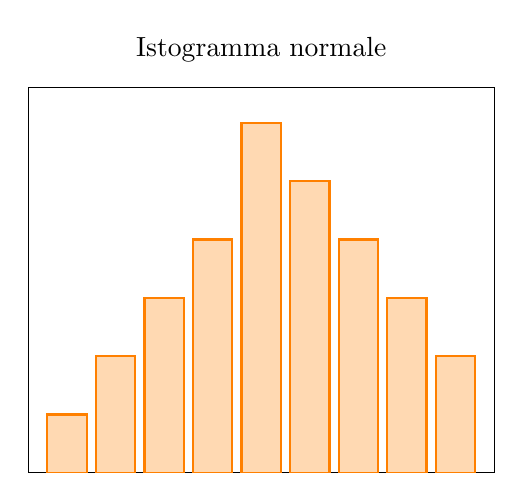
\begin{tikzpicture}
		\begin{axis}[
				title={Istogramma normale},
				xtick=\empty,
				ytick=\empty,
				ymin=0,
				width=7.5cm,
				ybar,
				bar width=0.5cm,
				grid=both,
				grid style=dashed
			]

			\addplot [
				thick,
				draw=orange,
				fill=orange!30,
			]
			coordinates {(0, 1) (1, 2) (2, 3) (3, 4) (4, 6) (5, 5) (6, 4) (7, 3) (8, 2)};
		\end{axis}
	\end{tikzpicture}
	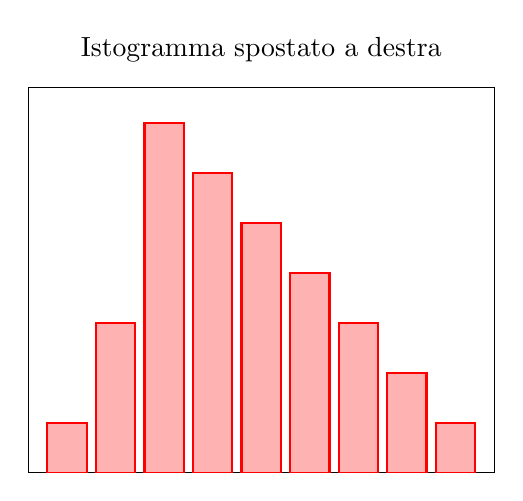
\begin{tikzpicture}
		\begin{axis}[
				title={Istogramma spostato a destra},
				xtick=\empty,
				ytick=\empty,
				ymin=0,
				width=7.5cm,
				ybar,
				bar width=0.5cm,
				grid=both,
				grid style=dashed
			]
			\addplot [
				thick,
				draw=red,
				fill=red!30,
			] coordinates {(0, 1) (1, 3) (2, 7) (3, 6) (4, 5) (5, 4) (6, 3) (7, 2) (8, 1)};
		\end{axis}
	\end{tikzpicture}

	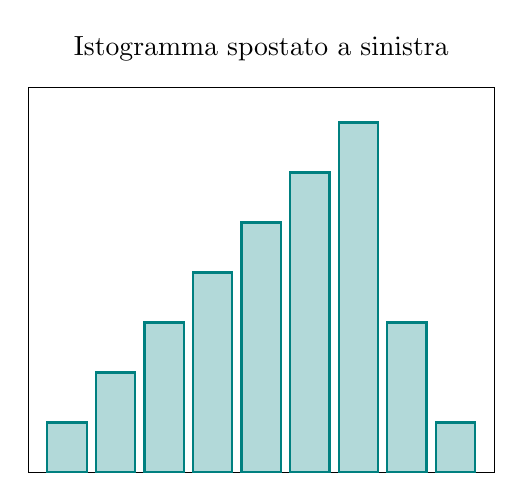
\begin{tikzpicture}
		\begin{axis}[
				title={Istogramma spostato a sinistra},
				xtick=\empty,
				ytick=\empty,
				ymin=0,
				width=7.5cm,
				ybar,
				bar width=0.5cm,
				grid=both,
				grid style=dashed
			]

			\addplot [
				thick,
				draw=teal,
				fill=teal!30,
			]
			coordinates {(0, 1) (1, 2) (2, 3) (3, 4) (4, 5) (5, 6) (6, 7) (7, 3) (8, 1)};
		\end{axis}
	\end{tikzpicture}
	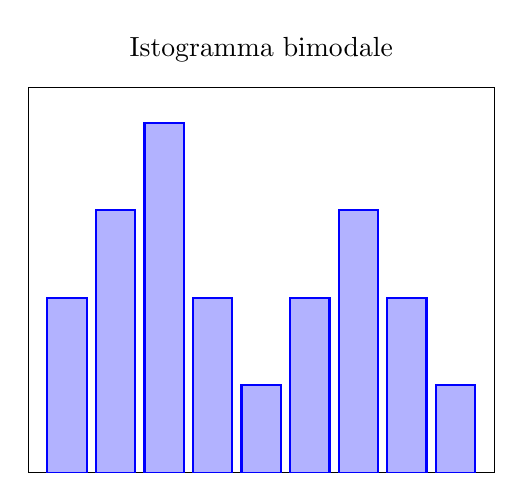
\begin{tikzpicture}
		\begin{axis}[
				title={Istogramma bimodale},
				xtick=\empty,
				ytick=\empty,
				ymin=0,
				width=7.5cm,
				ybar,
				bar width=0.5cm,
				grid=both,
				grid style=dashed
			]
			\addplot [
				thick,
				draw=blue,
				fill=blue!30
			]
			coordinates {(0, 2) (1, 3) (2, 4) (3, 2) (4, 1) (5, 2) (6, 3) (7, 2) (8, 1)};
		\end{axis}
	\end{tikzpicture}
\end{center}